\documentclass[12pt,a4paper]{article}

\usepackage[T1,T2A]{fontenc}
\usepackage[utf8]{inputenc}
\usepackage[english, russian]{babel}
\usepackage{indentfirst}
\usepackage{misccorr}
\usepackage{graphicx}
\usepackage{amsmath}
\usepackage{graphicx}
\usepackage{float}
\usepackage[left=20mm,right=10mm, top=20mm,bottom=20mm,bindingoffset=0mm]{geometry}

\setlength{\parskip}{6pt}
\DeclareGraphicsExtensions{.png}

\begin{document}

    \begin{titlepage}
        \begin{center}
            \large
            Санкт-Петербургский политехнический университет\\Петра Великого\\
            \vspace{0.5cm}
            Институт прикладной математики и механики\\
            \vspace{0.25cm}
            Кафедра «Прикладная математика»
            \vfill
            \textsc{\LARGE\textbf{Отчет по лабораторной работе №4}}\\[5mm]
            \Large
            по дисциплине\\"Математическая статистика"
        \end{center}
        \vfill
        \begin{tabular}{l p{175} l}
            Выполнила студентка\\группы 3630102/80201 && Деркаченко Анна Олеговна
            \vspace{0.25cm}
            \\Проверил\\доцент, к.ф.-м.н. && Баженов Александр Николаевич
        \end{tabular}
        \vfill
        \begin{center}
            Санкт-Петербург\\2021 г.
        \end{center}
    \end{titlepage}

\newpage
\begin{center}
    \tableofcontents
    \setcounter{page}{2}
\end{center}
\newpage
\begin{center}
    \listoffigures
\end{center}

\newpage
\section{Постановка задачи}
Даны распределения:
\begin{itemize}
    \item нормальное распределение $N(x,0,1)$
    \item распределение Коши $C(x,0,1)$
    \item распределение Лапласа $L(x,0,\frac{1}{\sqrt{2}})$
    \item распределение Пуассона $P(k,10)$
    \item равномерное распределение $U(x,-\sqrt{3},\sqrt{3})$
\end{itemize}

Необходимо:
\begin{enumerate}
    \item Сгенерировать выборки размером 20, 60 и 100 элементов
    \item Построить эмпирические функции распределения и ядерные оценки плотности распределения на отрезке $[-4, 4]$ для непрерывных распределений и на отрезке $[6, 14]$ для распределения Пуассона
\end{enumerate}

\section{Теория}
\subsection{Эмпирическая функция распределения}
\textit{Статистический ряд} - последовательность различных элементов выборки ${\{z_i\}}_{i=1}^k$, расположенных по восзрастанию, суказанием частот ${\{n_i\}}_{i=1}^k$, с которыми эти элементы содержатся в выборке.

\textit{Эмпирическая функция распределения} - относительная частота события $X<x$, полученная по данной выборке:
\begin{equation}
    F_n^*(x)=P^*(X<x)
\end{equation}

Ее можно найти по формуле:
\begin{equation}
    F^*(x)=\frac{1}{n}\sum_{z_i<x}n_i
\end{equation}
где $F^*(x)-$ функция распределения дискретной случайной величины $X^*$, заданной таблицей распределения:
\begin{table}[H]
    \centering
    \begin{tabular}{|c|c|c|c|c|}
        \hline
         $X^*$ & $z_1$ & $z_2$ & ... & $z_k$\\
         \hline
         $P$ & $\frac{n_1}{n}$ & $\frac{n_2}{n}$ & ... & $\frac{n_k}{n}$\\
         \hline
    \end{tabular}
    \caption{Таблица распределения}
\end{table}
Эмпирическая функция распределения является оценкой, т. е. приближённым значением, генеральной функции распределения $F_n^*(x)\approx F_X(x)$

\subsection{Ядерные оценки плотности вероятности}
\textit{Оценка плотности вероятности $f(x)$} - построенная на основе выборки функция $\widehat{f}(x):\widehat{f}(x)\approx f(x)$

Непрерывная ядерная оценка задается формулой:
\begin{equation}
    \widehat{f}_n(x)=\frac{1}{n h_n}\sum_{i=1}^n{K(\frac{x-x_i}{h_n})}
\end{equation}
где $K(u)$ - ядро, т. е. непрерывная функция, являющаяся плотностью вероятности, $x_1,...,x_n$ - элементы выборки, последовательность $\{h_n\}:$
\begin{equation}
    h_n\xrightarrow[n\to\infty]{}0;
    n h_n\xrightarrow[n\to\infty]{}\infty.
\end{equation}

Используется Гауссово ядро:
\begin{equation}
    K(u)=\frac{1}{\sqrt{2\pi}}e^{-\frac{u^2}{2}}
\end{equation}

А также правило Сильвермана:
\begin{equation}
    h_n=1.06\hat{\sigma}n^{-1/5}
\end{equation}
где $\hat{\sigma}$ - выборочное стандартное отклонение.

\section{Реализация}
Реализация лабораторной работы проводилась на языке Python в среде разработки PyCharm c использованием дополнительных библиотек:
\begin{itemize}
    \item scipy
    \item numpy
    \item math
    \item matplotlib
    \item seaborn
    \item statsmodels
\end{itemize}

Исходный код лабораторной работы размещен в GitHub-репозитории.

URL: https://github.com/derkanw/Mathstat/tree/main/lab4

\section {Результаты}
\subsection{Эмпирическая функция распределения}
\begin{figure}[H]
    \centering
    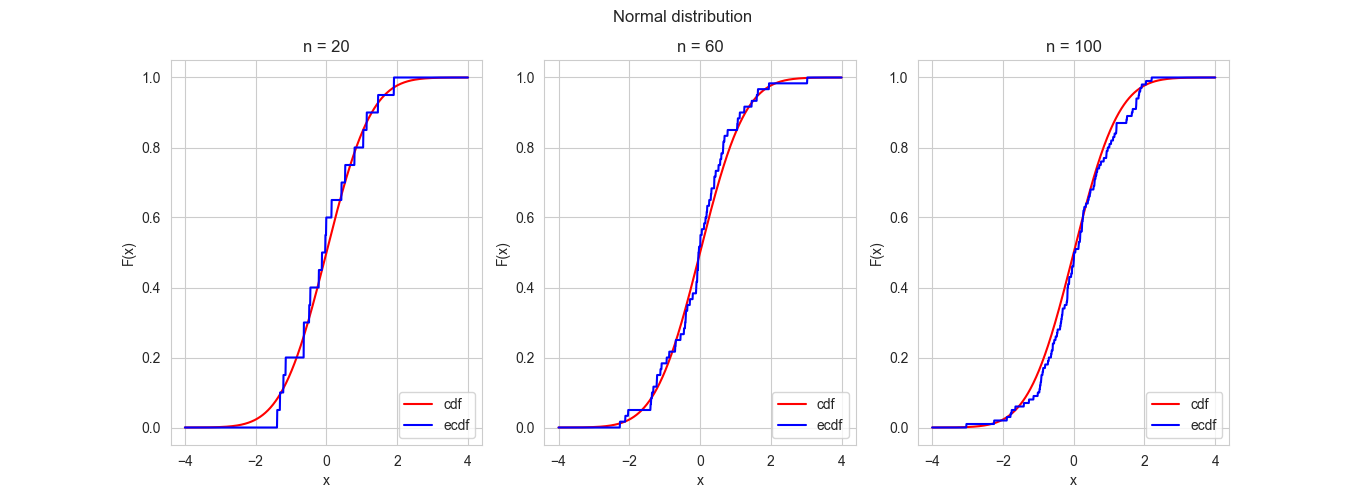
\includegraphics[scale=0.5]{images/Normal.png}
    \caption{Нормальное распределение}
\end{figure}

\begin{figure}[H]
    \centering
    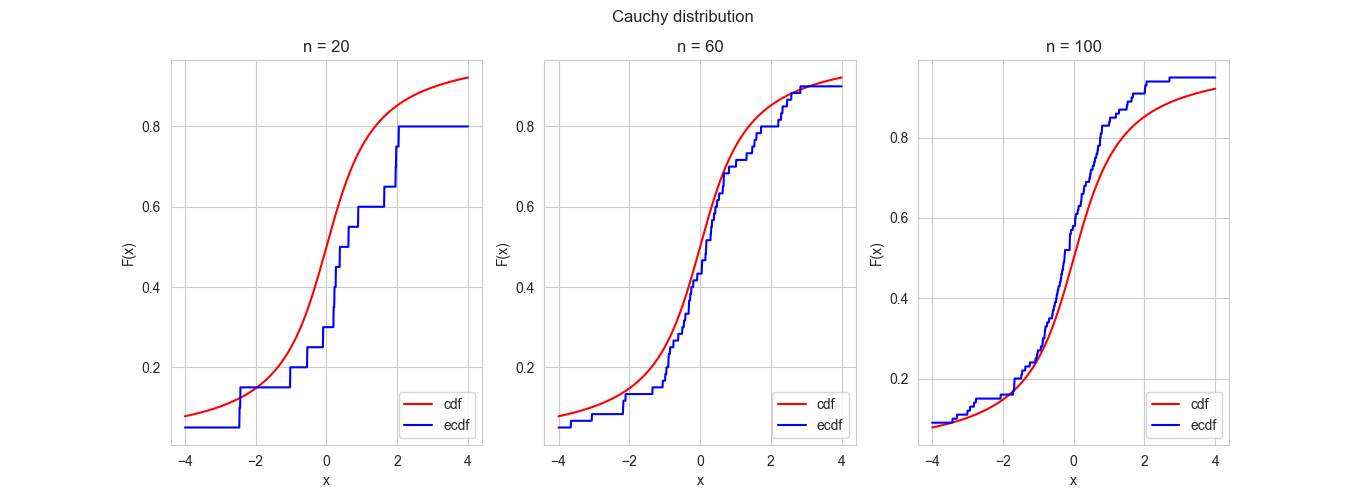
\includegraphics[scale=0.5]{images/Cauchy.png}
    \caption{Распределение Коши}
\end{figure}

\begin{figure}[H]
    \centering
    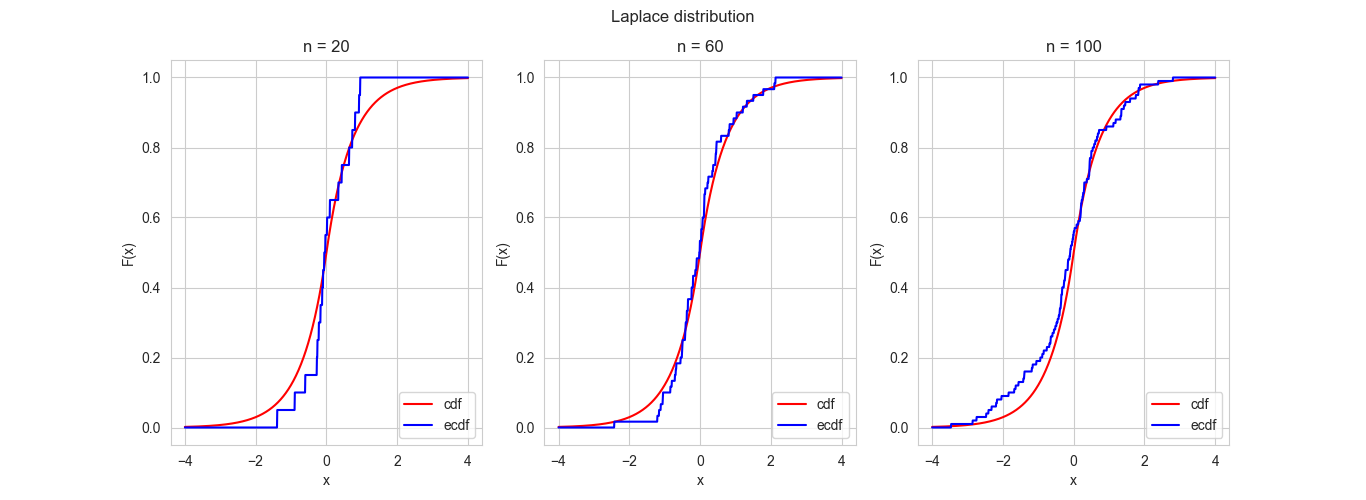
\includegraphics[scale=0.5]{images/Laplace.png}
    \caption{Распределение Лапласа}
\end{figure}

\begin{figure}[H]
    \centering
    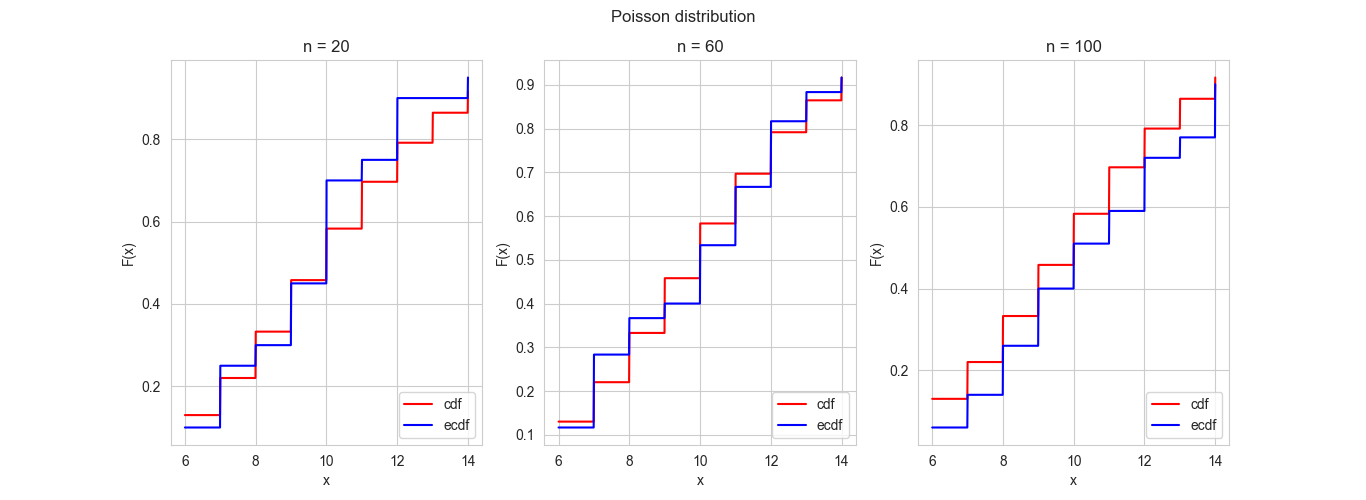
\includegraphics[scale=0.5]{images/Poisson.png}
    \caption{Распределение Пуассона}
\end{figure}

\begin{figure}[H]
    \centering
    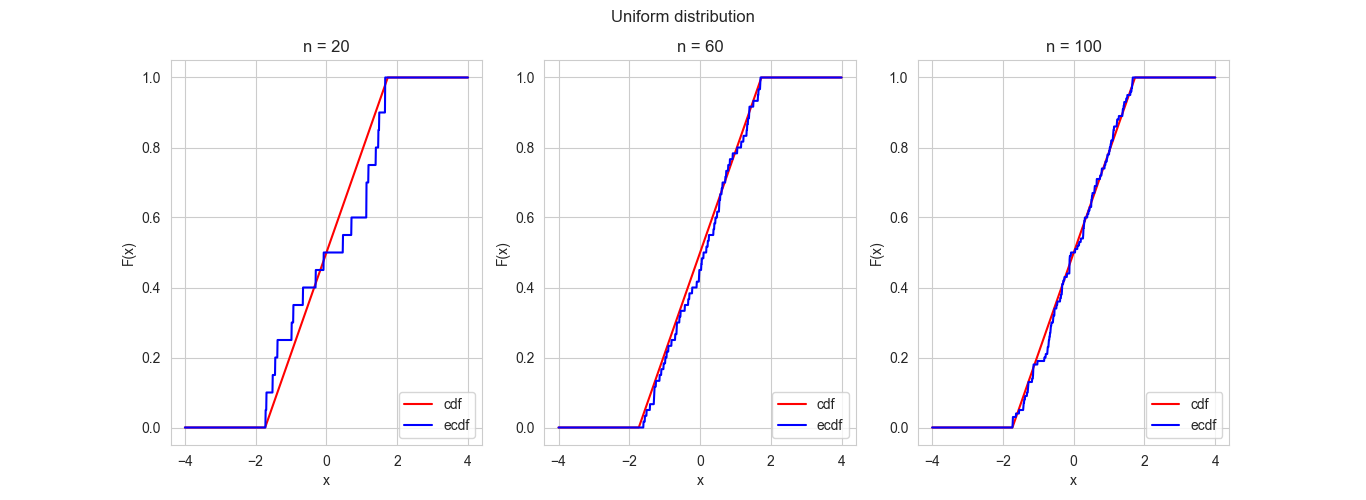
\includegraphics[scale=0.5]{images/Uniform.png}
    \caption{Равномерное распределение}
\end{figure}

\subsection{Ядерные оценки плотностей распределения}
\begin{figure}[H]
    \centering
    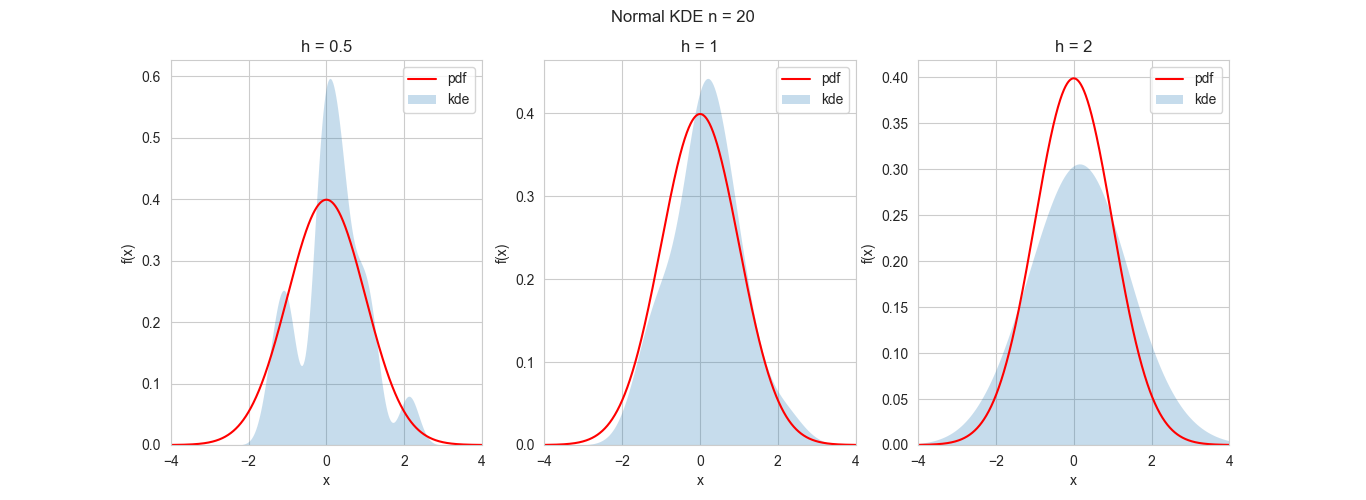
\includegraphics[scale=0.5]{images/Normal20.png}
    \caption{Нормальное распределение размерностью 20}
\end{figure}

\begin{figure}[H]
    \centering
    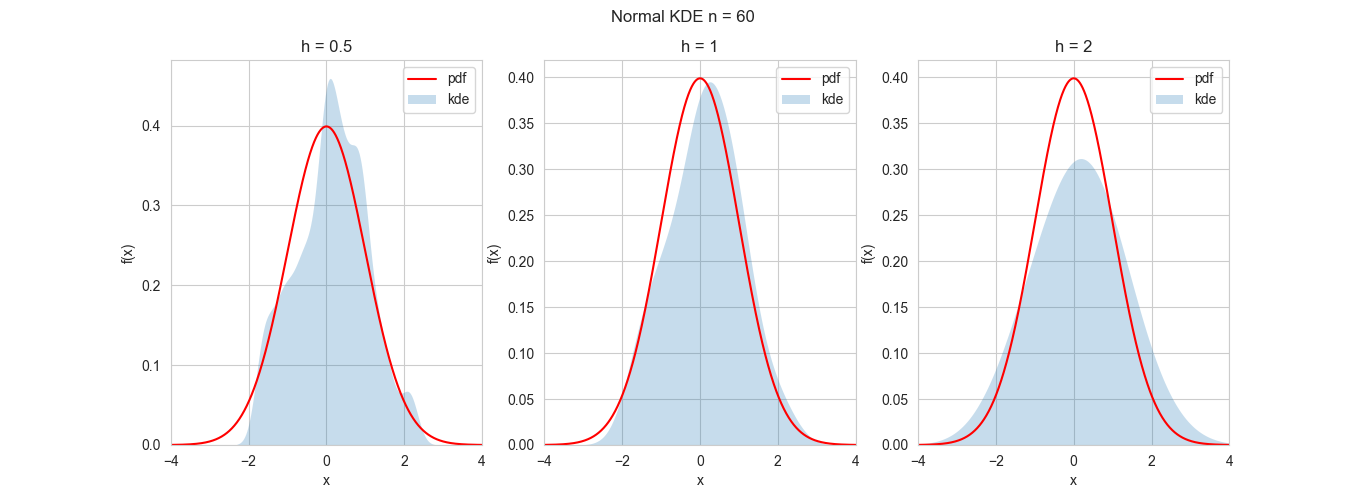
\includegraphics[scale=0.5]{images/Normal60.png}
    \caption{Нормальное распределение размерностью 60}
\end{figure}

\begin{figure}[H]
    \centering
    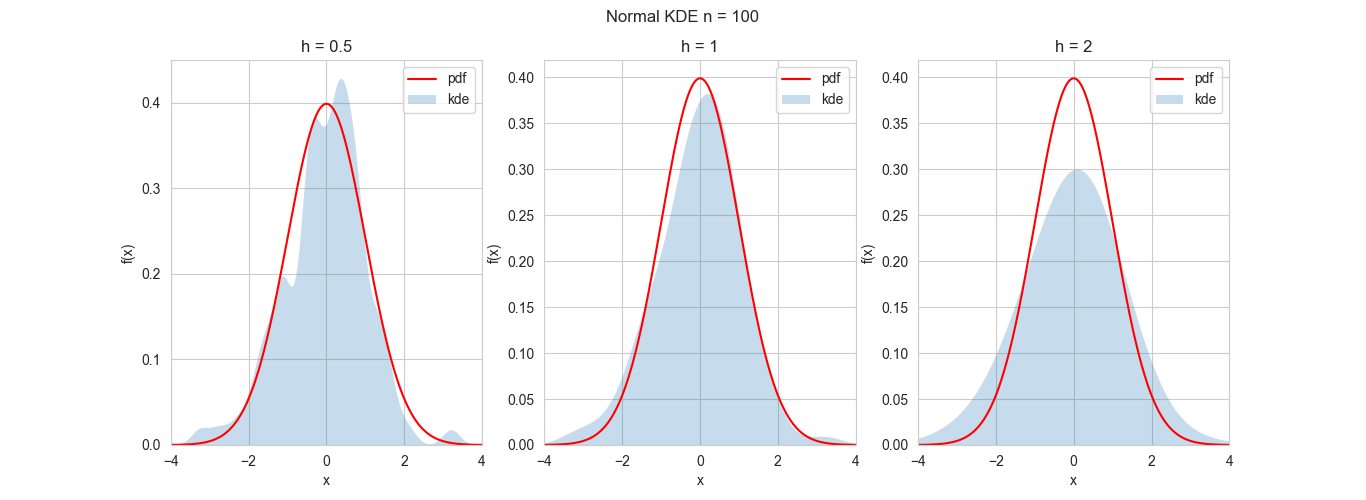
\includegraphics[scale=0.5]{images/Normal100.png}
    \caption{Нормальное распределение размерностью 100}
\end{figure}

\begin{figure}[H]
    \centering
    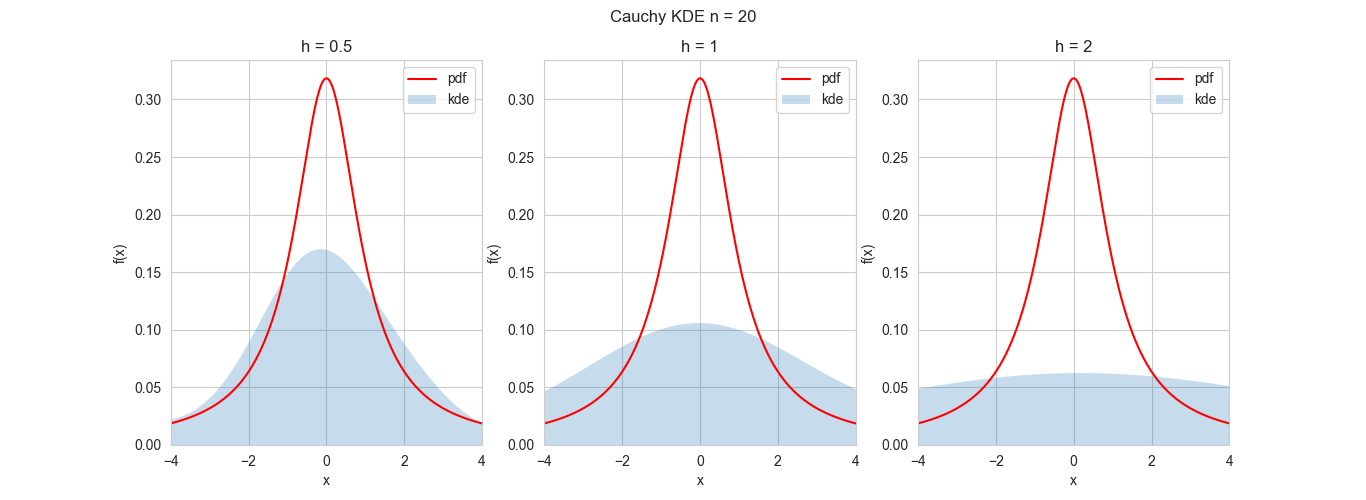
\includegraphics[scale=0.5]{images/Cauchy20.png}
    \caption{Распределение Коши размерностью 20}
\end{figure}

\begin{figure}[H]
    \centering
    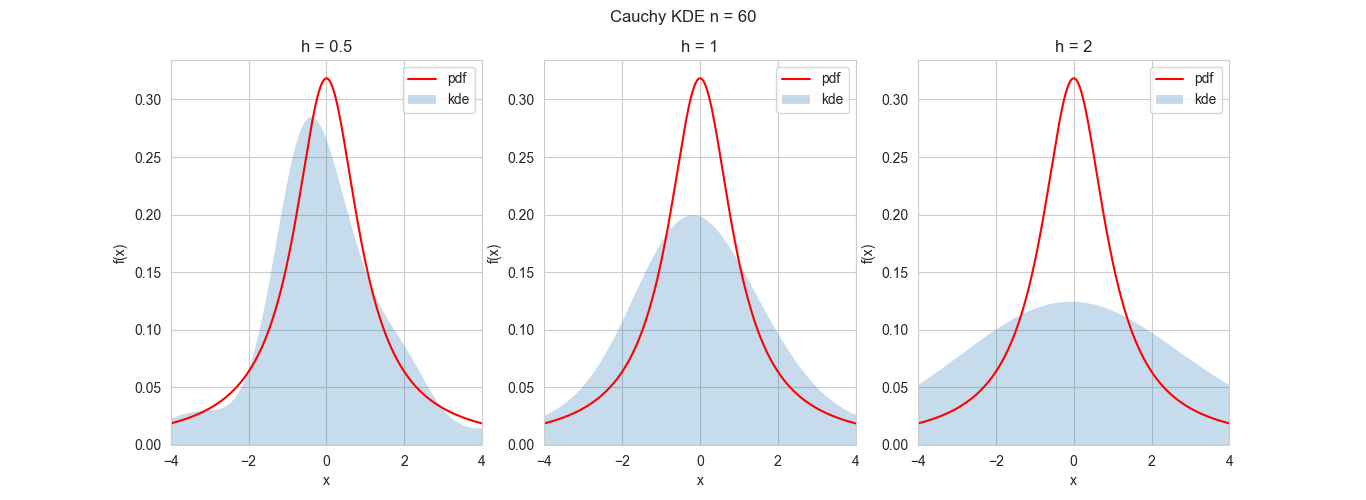
\includegraphics[scale=0.5]{images/Cauchy60.png}
    \caption{Распределение Коши размерностью 60}
\end{figure}

\begin{figure}[H]
    \centering
    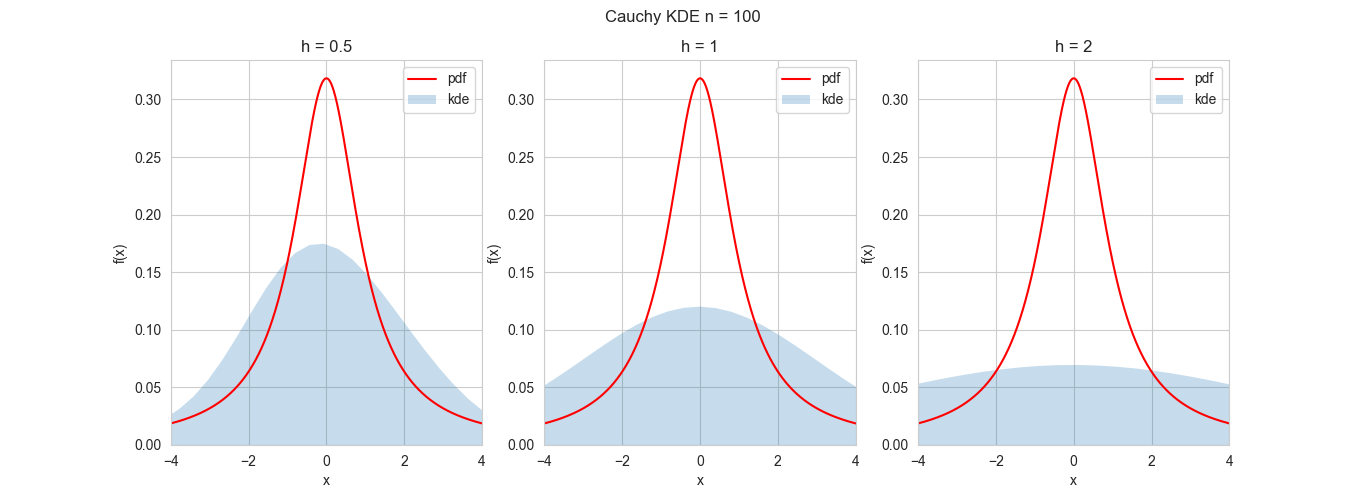
\includegraphics[scale=0.5]{images/Cauchy100.png}
    \caption{Распределение Коши размерностью 100}
\end{figure}

\begin{figure}[H]
    \centering
    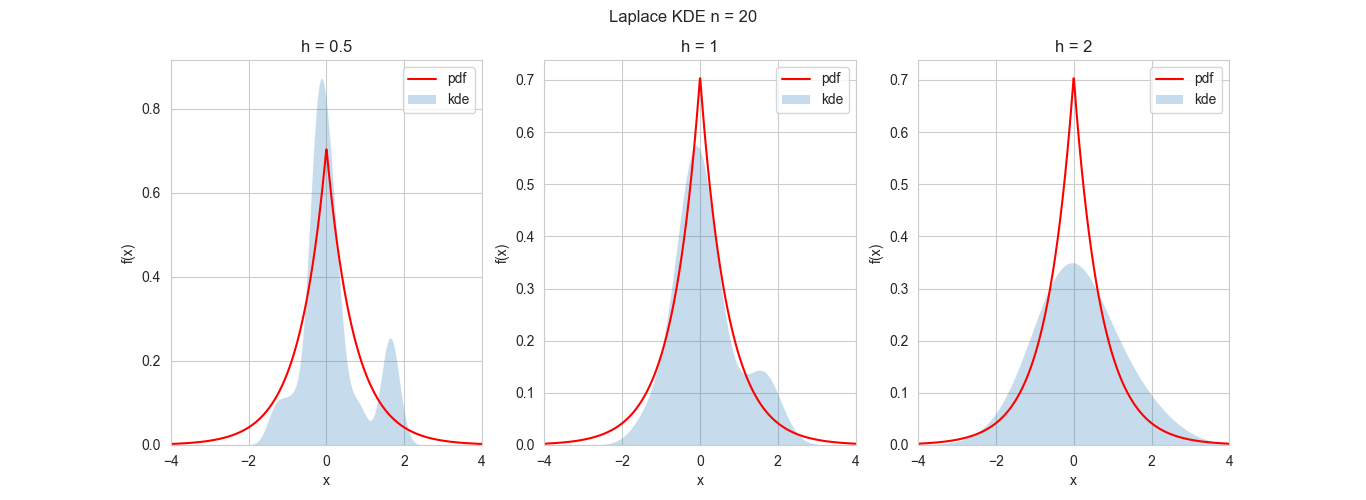
\includegraphics[scale=0.5]{images/Laplace20.png}
    \caption{Распределение Лапласа размерностью 20}
\end{figure}

\begin{figure}[H]
    \centering
    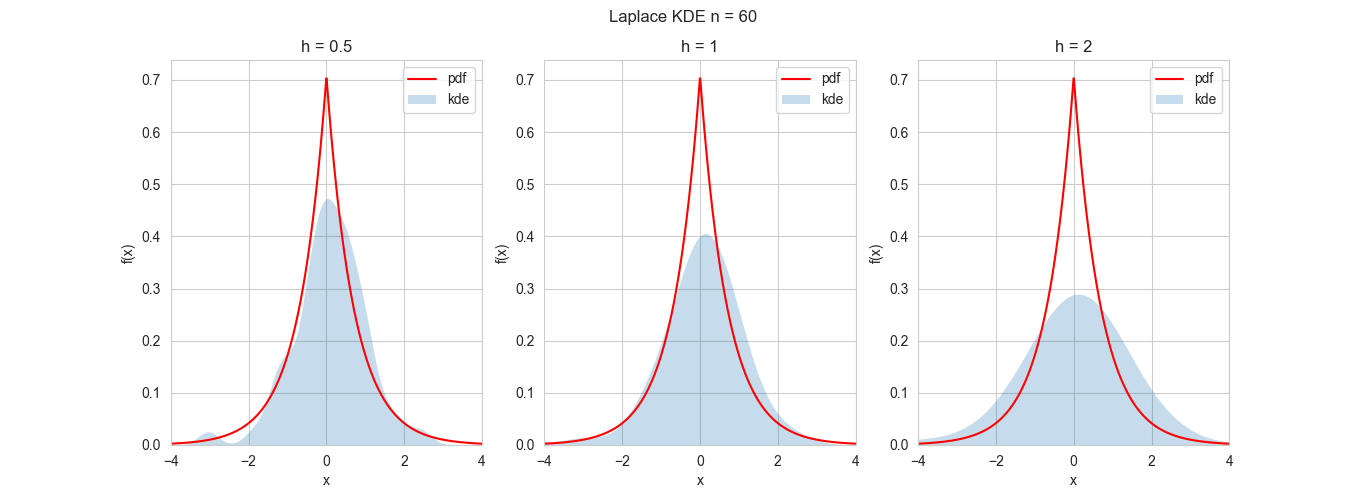
\includegraphics[scale=0.5]{images/Laplace60.png}
    \caption{Распределение Лапласа размерностью 60}
\end{figure}

\begin{figure}[H]
    \centering
    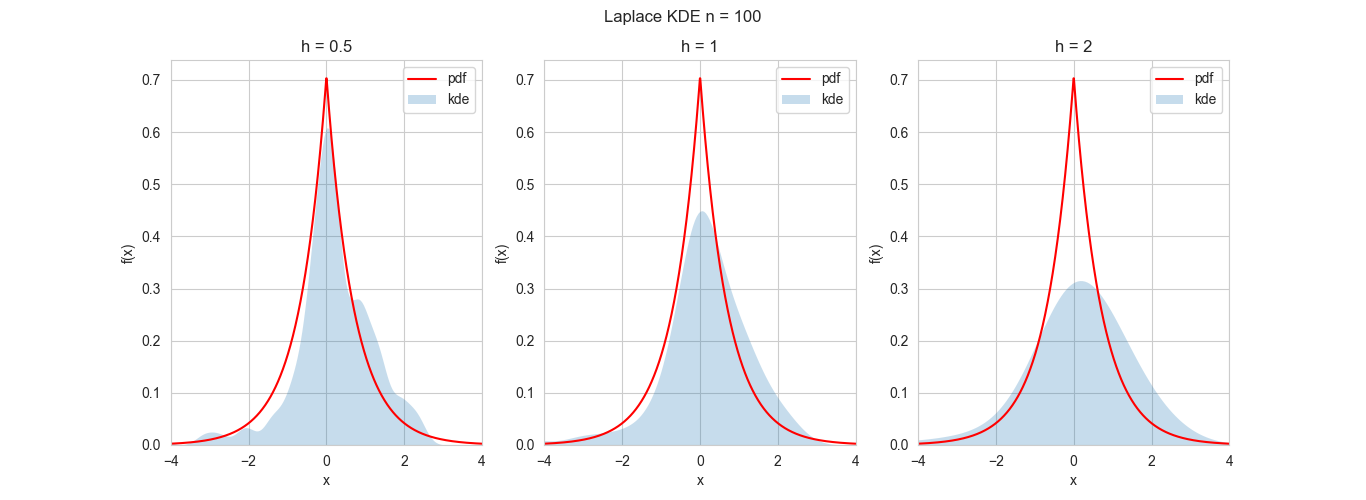
\includegraphics[scale=0.5]{images/Laplace100.png}
    \caption{Распределение Лапласа размерностью 100}
\end{figure}

\begin{figure}[H]
    \centering
    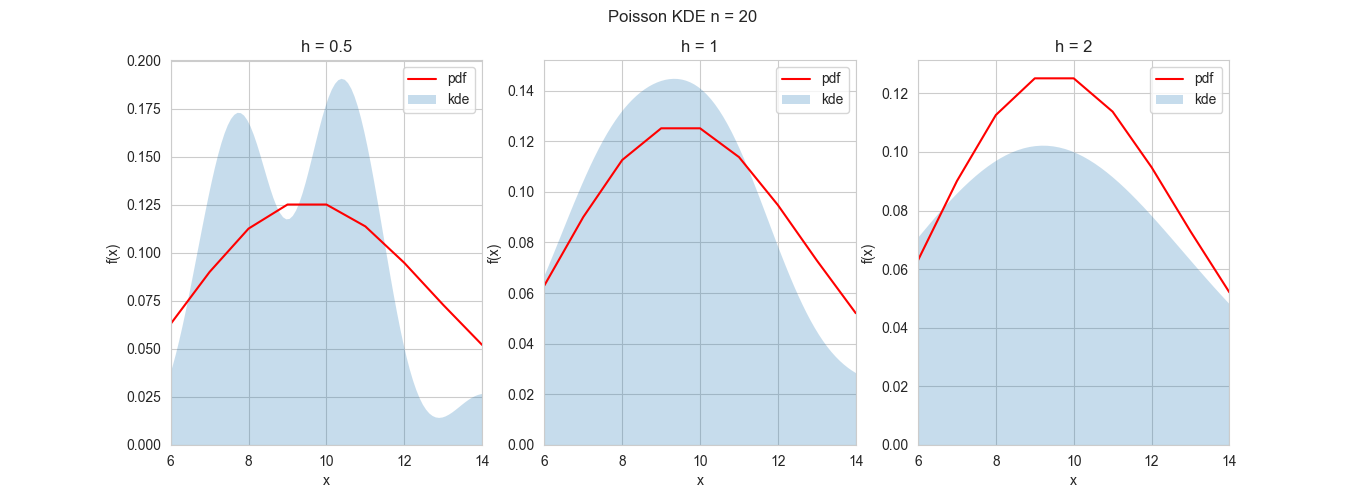
\includegraphics[scale=0.5]{images/Poisson20.png}
    \caption{Распределение Пуассона размерностью 20}
\end{figure}

\begin{figure}[H]
    \centering
    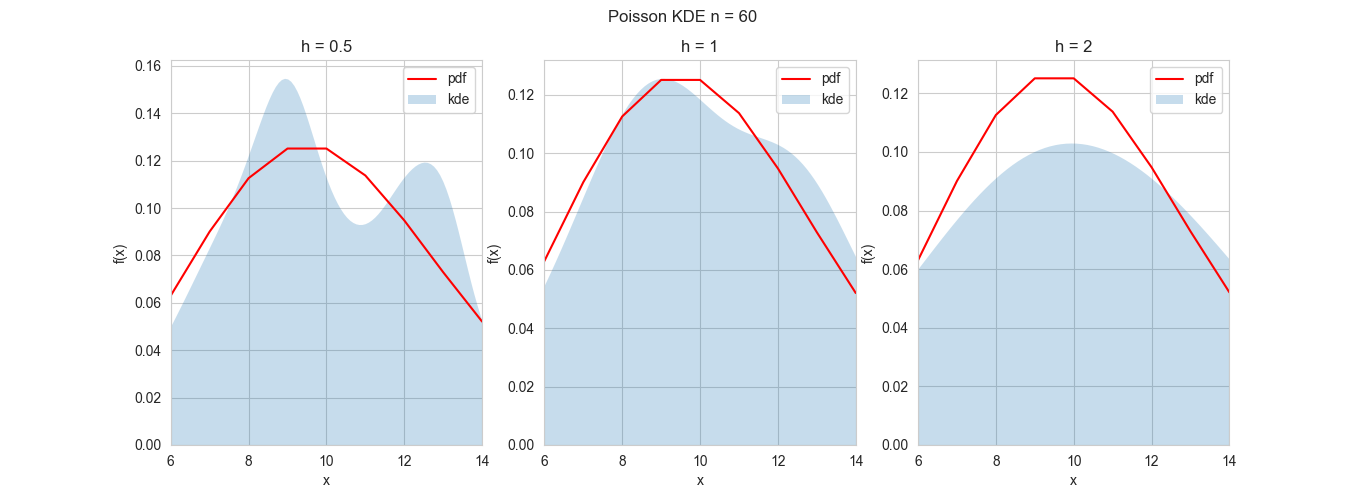
\includegraphics[scale=0.5]{images/Poisson60.png}
    \caption{Распределение Пуассона размерностью 60}
\end{figure}

\begin{figure}[H]
    \centering
    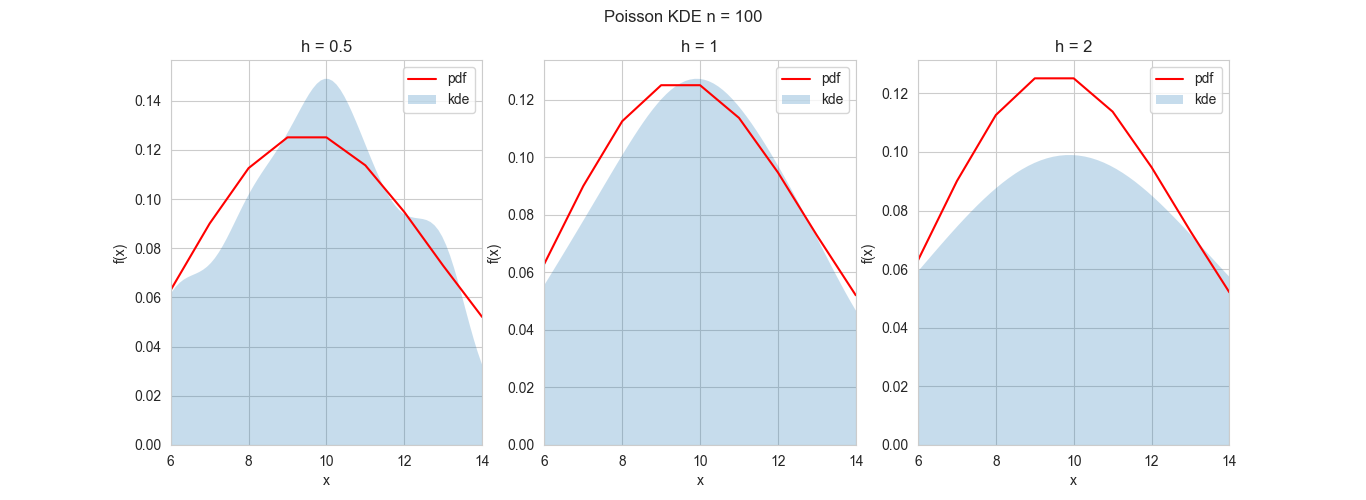
\includegraphics[scale=0.5]{images/Poisson100.png}
    \caption{Распределение Пуассона размерностью 100}
\end{figure}

\begin{figure}[H]
    \centering
    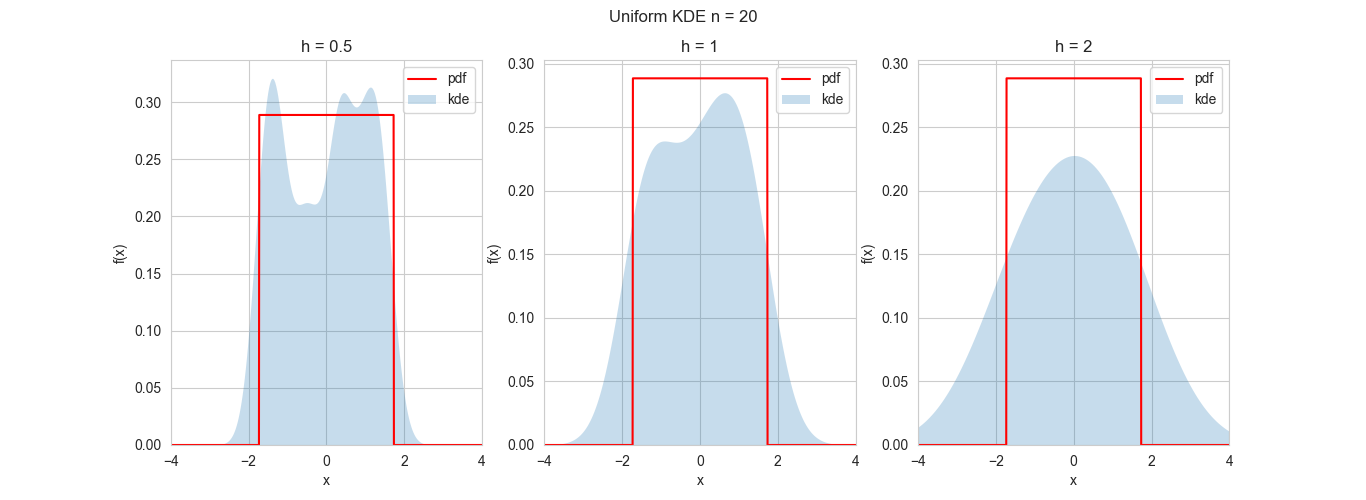
\includegraphics[scale=0.5]{images/Uniform20.png}
    \caption{Равномерное распределение размерностью 20}
\end{figure}

\begin{figure}[H]
    \centering
    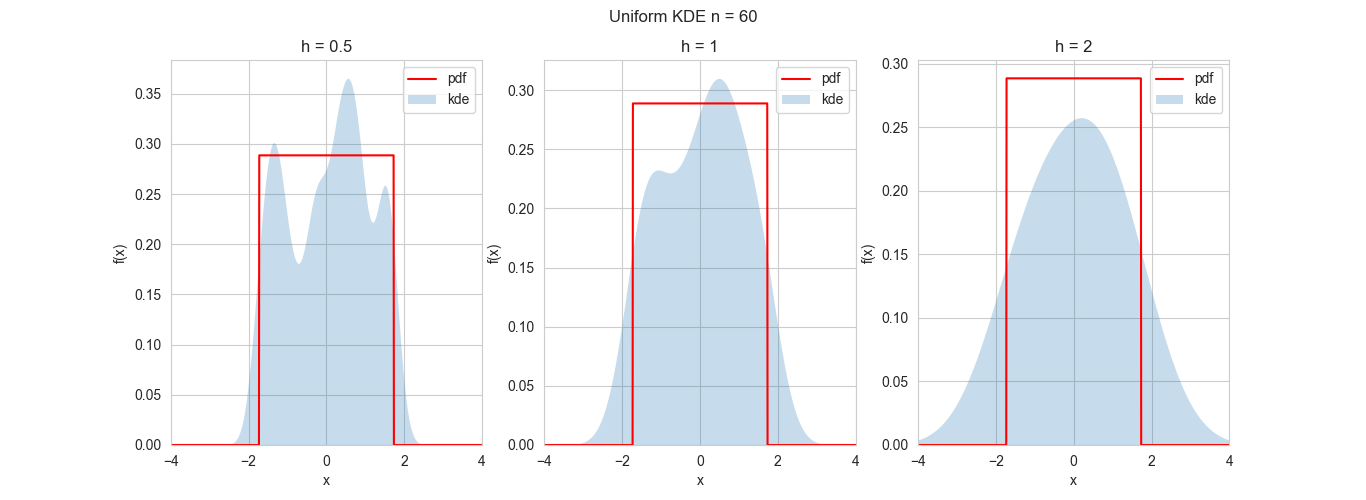
\includegraphics[scale=0.5]{images/Uniform60.png}
    \caption{Равномерное распределение размерностью 60}
\end{figure}

\begin{figure}[H]
    \centering
    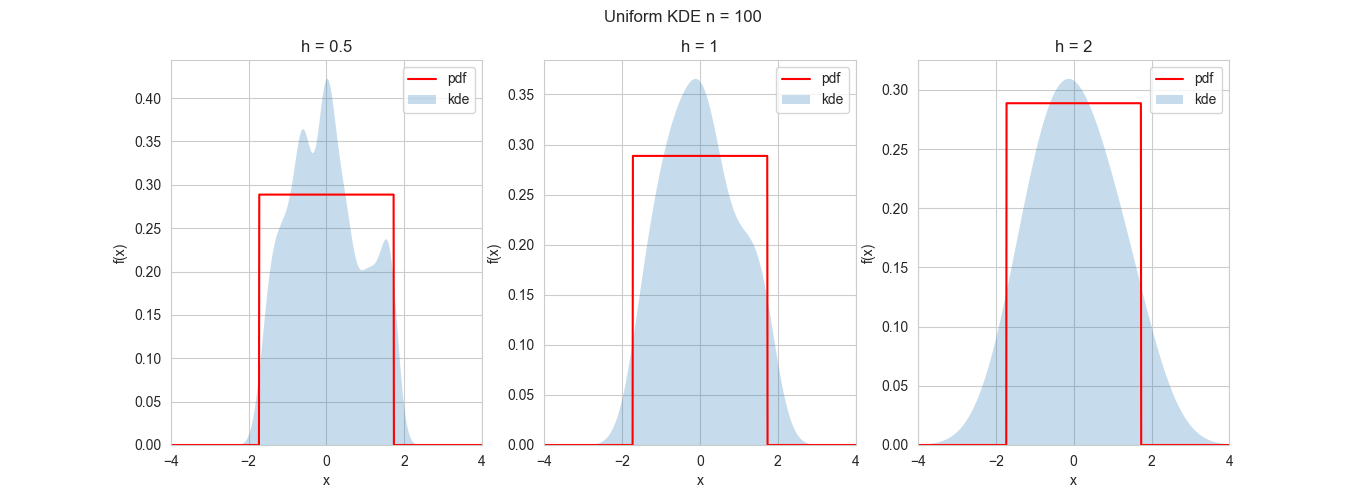
\includegraphics[scale=0.5]{images/Uniform100.png}
    \caption{Равномерное распределение размерностью 100}
\end{figure}

\section{Обсуждение}
При рассмотрении графиков эмпирических функций наблюдается следующая закономерность: чем больше размерность выборки, тем ступенчатая эмпирическая функция, построенная по ней, больше приближается к эталонной функции распределения данной величины. Стоит отметить, что для распределения Пуассона характерно наибольшее отклонение графика эмпирической функции распределения от эталонной.

Иллюстрации ядерных оценок плотностей распределения демонстрируют в большинстве случаев приближение ядерной оценки к функции плотности вероятности по всем $h$ с увеличением размерности выборки. Однако оптимальным значением для распределения Коши можно назвать размерность выборки, равной 60.

Для каждого из распределений оптимальным является свое значение параметра $h$. Параметр $h=h_n$ лучше всего приближает нормальное распределение, распределение Пуассона и равномерного распределение. Для распределения Коши и Лапласа оптимальным значением является $h=\frac{h_n}{2}$.

Также для распределения Коши и равномерного распределения при увеличении параметра $h$ характерно уменьшение значения пиковой точки и расширение основания графика ядерной оценки. А для всех распределений наблюдается преобразование графика ядерной оценки в функцию с единственным максимумом при значении параметра $h=2h_n$.
\end{document}
